\clearpage
\section{Motivations Behind LLM-Generated Code Detection}
Although it may seem exaggerated to begin the historical 
overview of code generation 
\hyperref[sec:Code_Generator]{Section 1.1.2} with compilers, 
this choice aims to emphasize that the present work does not 
seek to demonize the contribution or usefulness of code 
generation tools. It is undeniable that such tools are 
extremely valuable in both professional software development, 
accelerating simpler phases of implementation, and 
in educational contexts, where they can serve as 
useful assistants for learning how to write code.

Nevertheless, it is equally clear that is raising 
the need, in certain contexts 
and for specific reasons, to limit or discourage 
the use of highly advanced tools for code autocompletion 
or generation.

\vspace{1\baselineskip}
\noindent

One important reason concerns \textbf{academic and 
professional integrity}: the undeclared use of 
LLMs in evaluation contexts makes the assessment 
process highly problematic. Students, for example, 
may complete assignments or even exams using LLMs 
without contributing meaningfully to the generated 
code, potentially impairing their learning of 
fundamental programming concepts 
(getting the most out with the least effort). Similarly, 
during a technical interview, a candidate might 
rely on a tool like AlphaCode 2 to generate solutions 
to proposed problems.
This is the main topic of
\textit{"The Impact of Large Language Models on 
Programming Education…"} \cite{Jost2024LLM}
in which is demonstrated that a widespread use of 
LLMs code generator has negatively affects 
over students' capability.

Figure~\ref{fig:scatterplot} illustrates 
possible correlation between final grade and the
use of LLM. We can observe that an increase 
in LLM usage tends to correlate with lower 
average student grades, although it is not a 
decisive factor in determining the final score.

%Several studies raise concerns about these issues, 
%including: 
%Demirok and Kutlu\ cite{demirok2025aigcodeset}, 
%Xu and Sheng \cite{xu2025codevision}, 
%Ye et al. \cite{ye2025uncovering}, 
%Orel, Azizov, and Nakov \cite{orel2025codetm4}, 
%Yang et al. \cite{yang2023zeroshot}, 
%Nguyen et al. \cite{nguyen2023snippet}, 
%Hoq et al. \cite{hoq2023detecting}, 
%Paek and Mohan \cite{paek2025java}, 
%Bulla et al. \cite{bulla2024excode}, 
%Pham et al. \cite{pham2023magecode}, 
%and Park et al. \cite{park2025paraphrased}.

\vspace{1\baselineskip}
\noindent

Another critical issue lies in the way LLMs generate code. 
Since these models are trained on massive corpora, 
evaluating the security and efficiency of the generated 
code is nearly impossible. The output may be 
\textbf{vulnerable or inefficient} 
due to subtle flaws that are hard to detect, especially 
when the code appears well-formatted and logically 
structured. 
This happens to overreliance on 
commonly seen patterns in the training corpus rather 
than more appropriate niche solutions.
The security issues are highlighted by the study
\textit{”Do Users Write More Insecure Code with AI Assistants?”} 
\cite{perry2022users}. This study shows a decrease in
code security simply by using an AI assistant instead of
traditional programming.

%Relevant studies that address this concern include: 
%Suh et al. \cite{suh2024empirical}, 
%Demirok and Kutlu \cite{demirok2025aigcodeset}, 
%Shi et al. \cite{shi2024between}, 
%Ye et al. \cite{ye2025uncovering}, 
%Rahman et al. \cite{rahman2024claude}, 
%Bulla et al. \cite{bulla2024excode}, 
%Orel et al. \cite{orel2025codetm4}, 
%Yang et al. \cite{yang2023zeroshot}, 
%Xu et al. \cite{xu2023perplexity}, 
%and Nguyen et al. \cite{nguyen2023snippet}.

\vspace{1\baselineskip}
\noindent

\textbf{Intellectual property} is yet another motivation 
for detecting LLM-generated code, a general problem 
in generative AI. This is not limited to the origin 
of training data but also concerns the risk that an 
LLM may reproduce copyrighted code, posing 
significant legal risks to software companies 
that could unknowingly integrate such code into 
their products.
This issue is not an exaggerated concern, 
it's a tangible risk \cite{DoeVGitHub2024}.

%This issue has been raised in several studies, 
%including Suh et al. \cite{suh2024empirical}, 
%Yang et al. \cite{yang2023zeroshot}, 
%Nguyen et al. \cite{nguyen2023snippet}, 
%Paek and Mohan \cite{paek2025java}, 
%Park et al. \cite{park2025paraphrased}, 
%and Rahman et al. \cite{rahman2024claude}.

\vspace{1\baselineskip}
\noindent

The least important reason, 
which directly 
concerns the development of code-oriented 
LLMs themselves, is the need to distinguish 
machine-generated code in training datasets. 
If a model is trained on LLMs' code we might run into
a general LLM code oriented \textbf{Model Collapse}. 
Indeed, training LLM on LLMs' code serves to deteriorate the 
output diversity and adaptability to real-world scenarios.
This feedback loop issue is addressed for example in 
\textit{"The curse of recursion…"} 
\cite{shumailov2023curse}.
If no method exists to detect such code, the 
datasets used for training future models would 
have to be limited to code written before the 
widespread availability of LLMs, in order to 
avoid contamination. This would result in 
code generation models being trained on 
increasingly outdated data. 


% This issue is notably highlighted by Orel, 
% Orel, Azizov, and Nakov~\cite{orel2025codetm4}.

%%% Figura studenti
\begin{figure}[H]
    \centering
    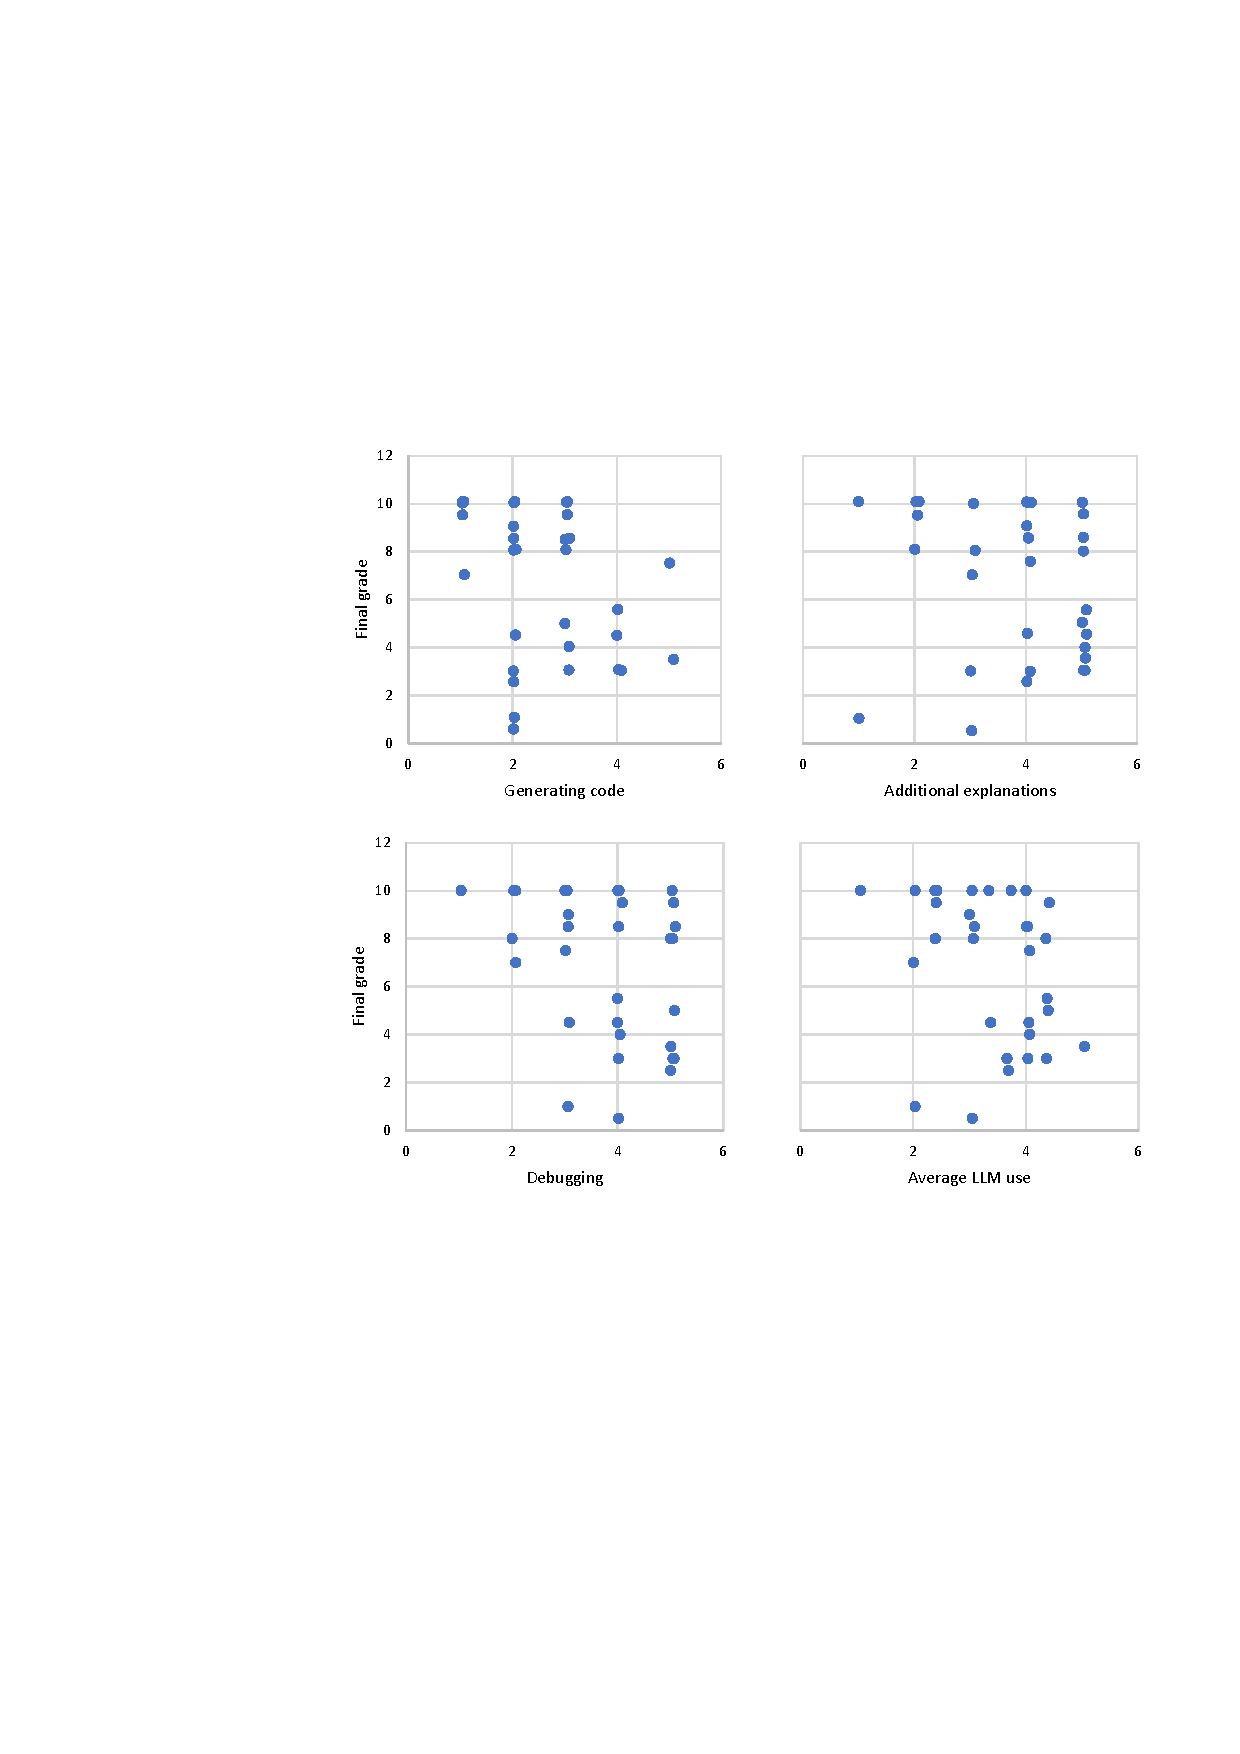
\includegraphics[width=0.9\textwidth]{img/1/scatterplot.pdf}
    \caption{Scatter plot from the paper 
        \emph{The Impact of Large Language 
        Models on Programming Education and 
        Student Learning Outcomes}, 
        illustrating the relationship between 
        LLM usage and students' final performance.}

    \label{fig:scatterplot}
\end{figure}